% !TEX root = ../main.tex

%tools
% \newcommand{\souffle}{\textsc{Souffl\'{e}}\xspace}
% \newcommand{\vampire}{\textsc{Vampire}\xspace}
% \newcommand{\eprover}{\textsc{E}\xspace}
% \newcommand{\spass}{\textsc{Spass}\xspace}

\newcommand{\souffle}{Souffl\'{e}\xspace}
\newcommand{\vampire}{Vampire\xspace}
\newcommand{\eprover}{E\xspace}
\newcommand{\spass}{Spass\xspace}


%languages
% \newcommand{\Datalog}{\textsc{Datalog}\xspace}
\newcommand{\Datalog}{Datalog\xspace}

%datalog notation
% \mathchardef\mhyphen="2D
% \makeatletter
% \newcommand*{\rl}{\mathrel{\texttt{:}\hspace{-0.075em}\mhyphen}}
% \makeatother
\newcommand*{\rl}{\mathrel{\leftarrow}}
\newcommand*{\comma}{\mathrel{\wedge}}

\renewcommand*{\phi}{\varphi}

\newcommand{\typedRel}[1]{\mathit{#1}}
\newcommand{\typed}[2]{\typedRel{#1}({#2})}

% Notation for Horn clauses definitions
\newcommand{\pred}[1]{\mathit{#1}} % predicates
\newcommand{\const}[1]{\mathrm{#1}} % constants
\newcommand{\type}[1]{\mathrm{#1}} % types

\newcommand{\sem}[1]{(#1)} % types

%qed
\def\eolqed{\hspace{\stretch1}\ensuremath\qedsymbol}

\newcommand{\PS}[1]{\textcolor{blue}{PS: {{#1}}}}

%-------------------------------------------------------------------------------
\section{Introduction}
\label{sect:aws/introduction}
Computer networks are typically built from a variety of specialized heterogeneous devices running complex distributed 
protocols. Network administrators, responsible for operability of a network, must configure and deploy every protocol 
separately on each individual device. In an effort to simplify this task, \emph{software-defined networking} (SDN)~\cite{SDN} 
has been proposed as a modern alternative. SDN provides an layer of software that is installed on each of the network 
devices and a logically-centralized controller that manages connectivity settings of each device. Administrators can 
therefore manage networks at a higher level of abstraction by programming them from the controller, typically in a domain 
specific language~\cite{DBLP:journals/cm/FosterGRSFKMRRSWH13}. The SDN architecture is often credited with flexibility and ease 
of maintenance compared to traditional networks~\cite{benzekki2016software}.

Modern platforms for cloud computing such as Amazon Elastic Compute Cloud, Google Compute Engine and Azure Virtual Machines offer their users means of configuring \emph{virtual private networks} in the style of SDN. Administrators of such networks use a centralized control panel or a specialized API to launch network instances, set up subnets and route tables, and tune connectivity and security settings of the network. Despite the increase of usability provided by the cloud platforms, virtual private networks remain prone to misconfigurations. These 
misconfigurations are caused by the complexity of large-scale enterprise networks and might lead to downtimes and breaches of 
security. Discovering such misconfiguration in industrial-sized networks can be both extremely labor and computationally intensive. Therefore, 
verifying the correctness of network configurations is an important and challenging task.

The presense of a centralized network configuration facilitates automated analysis of SDN networks. Indeed, several tools have been 
developed~\cite{batfish,jayaraman2014automated,DBLP:conf/icdcit/BjornerJ15,DBLP:conf/pldi/BallBGIKSSV14,Veriflow,ConfigChecker,Anteater,DBLP:conf/cav/El-HassanyTVV17} in an effort to verify various SDN components. These tools employ specialized algorithms~\cite{Veriflow} as well as general purpose 
reasoning engines such as 
\Datalog~\cite{muZ, DBLP:conf/cav/El-HassanyTVV17}, BDD~\cite{ConfigChecker}, SMT~\cite{jayaraman2014automated,DBLP:conf/icdcit/BjornerJ15} 
and SAT~\cite{Anteater,DBLP:conf/pldi/BallBGIKSSV14}.

%
% Problem 1: Size of networks, \Datalog works good in this however certain subproblems are hard for datalog
%
Despite the vast body of available tools, the problem of practical verification of enterprise networks still remains a 
challenge. Firstly, the size and intricacy of modern industrial-sized networks results in very difficult constraint 
satisfaction problems. While most network verification 
tools depend on a single constraint solving paradigm, we find that no single solver achieves best performance on all 
verification problems. Secondly, general purpose solvers are very 
performance-sensitive to problem encodings. Effective encodings are often a ``black art'' for users, resulting in tedious trial 
and error by the user without a good understanding of the implementation of the underlying solver.

%
% Explain our approach and tie back to in a nutshell how we solve problems 1 and 2
%
In this work we verify configurations of Amazon~VPC networks. The traffic flow in Amazon VPC networks is controlled by the rules assigned to various networking components available in Amazon~VPCs~\cite{WhatIsAmazonVPC}. These components include elastic network interfaces (ENI), subnets, and internet gateways. We are interested in checking \emph{network reachability properties}, that is, properties that express whether the network traffic is able to flow between given instances in an Amazon~VPC network.

We check reachability properties of Amazon~VPC networks using a portfolio of constraint solvers. To this end, we build static models of Amazon networks, translate the properties of these models to constraint satisfaction problems, and solve them using \Datalog engines and automated theorem provers for first-order logic.

Our motivation for using a portfolio of solvers rather than a single solver is to leverage the advantages of different types of solvers on different types of properties. \Datalog's strength lies in its efficient fixpoint computation and 
ability to efficiently store data, thus making it an efficient solver for listing all solutions~\cite{beliefs}. On the other hand, 
saturation based solvers exhibit superior performance on verification problems requiring large amounts of boolean reasoning. To 
maximize performance of both solvers, we translate each constraint satisfaction problem with the chosen solver in mind, thus 
facilitating greater scalabitity, i.e., solver computation speed and memory usage. We demonstrate the effectiveness 
of our approach by presenting a detailed evaluation of the both backend solvers. The results qualitatively confirm the complementary 
nature of the two backends, and show the ability of our tool to scale to large real-world VPC configurations.

% Overall Architecture of Tool
Our contributions are summarized as follows: \begin{enumerate*}[label=(\roman*)]
% \item We describe the overall architecture of our tool 
\item We explore efficient encodings for two types of backend solvers, including 
saturation-based solvers, which to the best of our knowledge, have not been used to verify networks
\item We provide a comparison of the backend solvers and classify their strengths and weaknesses
\end{enumerate*}.

The rest of the paper is organized as follows. Section~\ref{sect:aws/specification} describes the network reachability properties and the network models. Sections \ref{sect:aws/datalog}, and \ref{sect:aws/fol} present our translations of network properties for \Datalog engines, SMT solvers, and first-order theorem provers. Section~\ref{sect:aws/experiments} presents experimental results obtained by running constraint solvers on problems which we constructed from a collection of network configurations. Section~\ref{sect:aws/related} presents related work, and Section~\ref{sect:aws/conclusion} contains a discussion of this work and suggests future work.

%-------------------------------------------------------------------------------
%\section{Network Reachability}
%\label{sect:reachability}

\section{Motivation}
\label{sect:aws/motivation}
% \begin{figure}
% \includegraphics[width=0.36\textwidth]{./fig/system.pdf}
% \centering
% \caption{Tool Architecture\label{ex:tool}}
% \end{figure}

Let us motivate the problem of verifying virtual private networks using the following example of a network.
\begin{figure*}[th]
\centering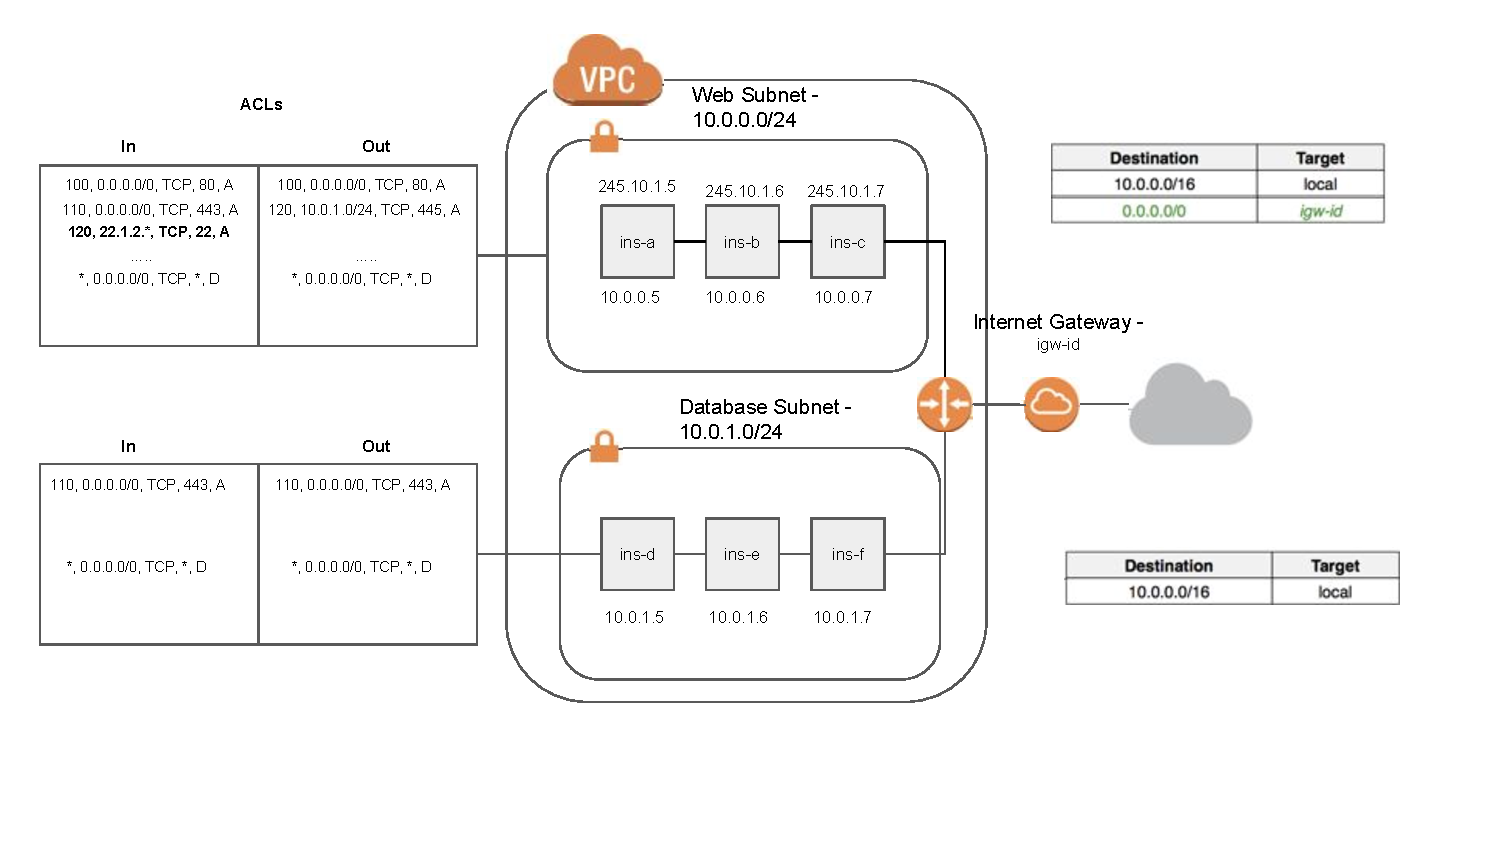
\includegraphics[width=1.0\textwidth]{./aws/fig/vpc.pdf}
\end{figure*}

This network consists of two subnets ``Web'' and ``Database'' and three network instances in each of them. Each of the subnets is assigned with a route table (on the right) and an access control list (ACL, on the left). The route tables allow the network traffic to flow between the subnets and between the ``Web'' subnet and the internet gateway. In other words, the network instances in the ``Web'' subnet are accessible from the internet. An ACL consists of rules that filter the network traffic to and from its subnet. In our example, one of the ACL rules of the ``Database'' subnet forbids SSH access to its instances, both directly and through an intermediate instance.

In a realistic setting this network might grow over time, obtaining more network instances and new security and access rules. A network administrator may want to make sure that the network retain certain properties after each change in its configuration. For example, the network administrator may want to check the following property.
\begin{example}\label{prop:bool-property}
All network instances in the subnet ``Web'' can access all network instances in the subnet ``Database''.
\end{example}

In addition, the network administrator might want to know which networking components satisfy a given property, such as the ones in the following example.
\begin{example}\label{prop:list-property}
All network instances that have the port 22 (SSH) accessible from the internet.
\end{example}

We will refer to questions that network administrators might want to answer, such as the ones in Examples~\ref{prop:bool-property} and \ref{prop:list-property}, as \emph{network questions}. In particular, we will refer to questions similar to Example~\ref{prop:bool-property} as \emph{boolean questions}, because they expect a true-or-false answer, and to questions similar to Example~\ref{prop:list-property} as \emph{list questions}, because they expect a list of networking components as an answer.

%
% Explain what we do in tiros
%
Answering network questions manually might be tedious and error-prone in an industrial-size network. For that reason this task is often automated with specialized tools. In this work we answer network questions by expressing them as constraint satisfaction problems and then solving these problems using a portfolio of constraint solvers.

We answer network questions using a combination of a \Datalog engines and automated theorem provers for first-order logic. We demonstrate that by using multiple types of constraint solvers we are able to pick the most appropriate solver for a given network question. This allows us to increase the overall efficiency of answering network questions. Consider the following example. Each boolean question can be equivalently phrased as a list question~--- the answer to the boolean question is true iff the answer to the correspondent list questions is not empty. However, we distinguish these two types of questions because, as we show later, we can more efficiently answer list questions with \Datalog engines and answer boolean questions with saturation-based theorem prover for first-order logic.

\EK{Also mention that we use two types of theorem provers to leverage the strengths of each one of them.}

%
% Explain the two types of properties and their suitability for different solvers
%
% We express the properties in many-sorted first-order logic and present their .
%
% Properties~\ref{prop:bool-property} and~\ref{prop:list-property} while being on the surface similar in nature, pose very different 
% challenges for constraint solvers. Property~\ref{prop:list-property} asks the tool to \emph{list} instances that can be accessed via 
% the internet. Solving this property involves monotonically computing the set of instances that via routes, ACLs, security groups etc. 
% can be accessed from the internet via an internet gateway connection. For such queries, \Datalog based solvers are very effective. In, 
% Property~\ref{prop:bool-property} can be rephrased as an assertion of the \emph{existence} of an instance in the Web subnet that cannot 
% access an instance in the Database subnet. Here, we find \Datalog solvers compute unnecessary information for the assertion. On the other 
% hand, saturation based solvers excel in this regard \PS{EK can you add why}.

% The goal of this work is to investigate the strengths and weaknesses of each backend and describe how their effective usage in an industrial 
% strength tool.

%are for solvers 
%Checking a property can be seen as a special case of discovering a set of networking components that satisfy this 
%property~--- the property holds iff the set is not empty. However, we distinguish these two problems because, as we show later, we can solve 
%them more efficiently using different types of constraint solvers.
%In order to check this property one needs to know the rules of the security groups, assigned to each network instance, the rules 
%of the network ACL, and the semantics of how these rules are enforced. Checking such reachability property involves reasoning 
%with constraints imposed by these networking components.
%In this work we are interested in checking a variety of properties e.g., whether the network traffic is able to flow between given 
%instances in an Amazon~VPC network.
%\PS{As already done below --explain what catch is with the queries and why we need two solvers}
%In addition to checking properties such as Example~\ref{example:bool-property}, we would like to discover the set of all networking 
%components that satisfy a given reachability property. For example, we would like to discover the following.
%\PS{the stuff below isn't so clear and doesn't flow} 
%We express the properties in many-sorted first-order logic and present their syntax and semantics in Section~\ref{sect:reachability/properties}.
%We check properties symbolically, i.e. instead of sending packets in a network, we build a model of the network and reason about this model. Our model consists of two parts, the \emph{specification} and the \emph{snapshot} of the network. The specification formalizes the semantics of each of the components available in the network. For example, the specification describes how a route table directs network traffic in a subnet or in which order a firewall applies rules in the access control list. The snapshot describes the topology of the given network. For example, the snapshot contains the list of network instances, subnets, and their route tables. Naturally, the specification in the model of each particular Amazon~VPC network is the same, whereas the snapshot differs. In the following section we present the syntax and semantics of our network models.

\PS{Dumping this here for now}
Our motivation for using \Datalog rests on its success in efficiently modeling
finite domain static analyses~\cite{doop}. While \Datalog was originally designed 
as a powerful database query language, there is a cornucopia of state-of-the-art \Datalog 
engines that are aimed at static analysis and treat \Datalog as a limited logic. Such tools 
have shown performance on a par with hand-crafted static analysis tools on large program 
analysis benchmarks~\cite{souffle}.

Unlike~\cite{beliefs}, we translate the network snapshot to the 
EDB, that is, a set of ground input relations. The networks semantics are converted into 
recursive and non-recursive \Datalog rules that and the user properties are converted into 
non-recursive chained rules. Our approach allows for us to take advantage of compilation and 
partial evaluation that is present in high performance \Datalog engines such as 
\souffle~\cite{souffle}.



\section{Network Reachability Properties}
\label{sect:aws/specification}
We answer network questions \emph{statically}, that is, instead of sending packets in a network, we build a model of the network and reason about this model. Our \emph{network model} consists of two parts, the \emph{formal specification} and the \emph{snapshot} of the network. The specification formalizes the semantics of each of the components available in the network. For example, the formal specification describes how a route table directs network traffic in a subnet or in which order a firewall applies rules in the access control list. The snapshot describes the topology of the given network. For example, the snapshot contains the list of network instances, subnets, and their route tables. Naturally, the formal specification in the model of each particular virtual private network is the same, whereas the snapshot differs. We express network questions in the language of many-sorted first-order logic. In the remainder of this section we describe syntax and semantics of network models and network questions.

\EK{We might want to make it clear that the models and the queries are given to us. Otherwise we'd have to justify why we use Datalog for the spec and FOL for the queries.}

\subsection{Network Models}
\label{sect:aws/reachability/spec}
We formally specify networks in a logic programming style. A network model is a finite set of first-order Horn clauses. We disallow function symbols and allow stratified negation. We assume the plain logic programming semantics for these Horn clauses, defined in the standard way~\cite{}. In particular, we make the closed-world assumption and treat negation as failure. In addition, our network models use the theory of bit vectors to describe ports, IPv4 addresses, and subnet masks.

A \emph{signature} of the network model is a triple $(T, C, P),$ where $T$ is a set of \emph{types}, $C$ is a set of \emph{constants}, and $P$ is a set of \emph{predicates}. We assign each constant with a type $\tau\in T$ and each predicate with a type $\tau_1\times\ldots\times\tau_n$ $(n\ge0)$, where $\tau_i\in T$ for each $1\leq i \leq n$. We assume a countable infinite set of \emph{variables}. We assign each variable with a type $\tau\in T$. We call a \emph{term} of the type $\tau\in T$ a constant or a variable of that type. We call an \emph{atom} an expression of the form $p(t_1,\ldots,t_n)$, where $n>0$, $p\in P$ is a predicate of the type $\tau_1\times\ldots\times\tau_n$, and each $t_i$, $1\leq i \leq n$ is a term of the type $\tau_i$. We call a \emph{literal} an atom or its negation.

A \emph{rule} is a Horn clause of the form $A\leftarrow L_1 \wedge \ldots \wedge L_n$ $(n \ge 0)$, where $A$ is an atom which we call the \emph{head} of the rule and each of $B_1,\ldots,B_n$ is a literal. If $n=0$ and all arguments of $A$ are constants then we call such rule a fact. We call a \emph{definition} of the predicate $p \in P$ the set of all rules in the network model that use $p$ in their head.

We assume that the signature contains
\begin{enumerate*}[label=(\roman*)]
  \item types $\type{bits16}$ and $\type{bits32}$;
  \item $2^{16}$ constants of the type $\type{bits16}$;
  \item $2^{32}$ constants of the type $\type{bits32}$;
  \item predicates $\pred{bits16}_<$, $\pred{bits16}_\le$, $\pred{bits16}_{+1}$, $\pred{bits16}_{-1}$ of the type $\type{bits16} \times \type{bits16}$ with a special semantics \EK{Careful! $\pred{bits16}_{+1}$ and $\pred{bits16}_{-1}$ are not total functions, mention that!}; and
  \item predicate $\pred{bits32}_\wedge$ or the type $\type{bits32}\times\type{bits32}\times\type{bits32}$ with a special semantics.
\end{enumerate*}
$\type{bits16}$ and $\type{bits32}$ represent the types of 16-bit and 32-bit vectors. The semantics of the predicates is that of the correspondent operations over bit vectors defined in the standard way.

We assume that for each type $\tau\in T$ the signature contains the equality predicate $\pred{=}_\tau$ of the type $\tau\times\tau$ and the network model contains the rule $\pred{=}_\tau(X,X)$.

The network specification part of the model contains types, predicates, constants, and rules that describe the semantics of the networking components in Amazon~VPCs. For example, the specification defines the semantics of SSH tunneling. One ENI can SSH tunnel to another ENI iff it can either connect to it over SSH directly, or through a chain of one or more intermediate ENIs. In order to express this concept, the specification contains predicates $\pred{canSshTunnel}$ and $\pred{canSsh}$, each of the type $\type{eni}\times\type{eni}$, and the two following rules.
\begin{align*}
\pred{canSshTunnel}(\mathit{Eni}_1,\mathit{Eni}_2)\leftarrow\:&\pred{canSsh}(\mathit{Eni}_1,\mathit{Eni}_2). \\
\pred{canSshTunnel}(\mathit{Eni}_1,\mathit{Eni}_2)\leftarrow\:&\pred{canSshTunnel}(\mathit{Eni}_1,\mathit{Eni}_3)\\
\wedge\:&\pred{canSshTunnel}(\mathit{Eni}_3,\mathit{Eni}_2).
\end{align*}
% can-ssh-tunnel-enis: eni * eni
% -: can-ssh-tunnel-enis Eni1 Eni2
% <- can-ssh-enis Eni1 Eni2.
% -: can-ssh-tunnel-enis Eni1 Eni2
% <- can-ssh-tunnel-enis Eni1 Eni3
% <- can-ssh-tunnel-enis Eni3 Eni2.

The specification of Amazon~VPC networks that we used in this work consists of approximately 50 types, 200 predicates, and over 240 rules.

The network snapshot part of the model contains constants and facts that describe the configuration of the networking components in a given Amazon~VPC network. For example, the snapshot of a network with a single instance \verb'i-abcd1234' in a single subnet ``Web'' consists of the constants $\const{instance}_\text{abcd1234}$ and $\const{subnet}_\text{Web}$, and the fact $$\pred{instanceHasSubnet}(\const{instance}_\text{abcd1234},\const{subnet}_\text{Web}).$$

\EK{Mention how large network snapshots get?}

\subsection{Network Questions}
\label{sect:aws/reachability/properties}

We express network questions as formulas of many-sorted first-order logic with the standard logical connectives $\vee$, $\wedge$, $\Rightarrow$, $\Leftrightarrow$, $\oplus$, and equality. These formulas only use types, constants, and predicates from the signature of the network model. The formulas do not use any function symbols. We allow interpretation of these formulas to use empty domains and otherwise assume the standard semantics of many-sorted first-order logic.

We express boolean questions as closed formulas, that is, formulas in which all variables are bound by a quantifier. Conversely, we express list questions as formulas with free variables. The answer to a boolean question is true iff its correspondent formula is valid. The answer to a list question is the set of substitutions of variable with constants that satisfy its correspondent formula.

The boolean question in Example~\ref{prop:bool-property} is expressed as the following formula.
\begin{equation}\label{eq:bool-property}
\begin{aligned}
&(\forall w:\type{instance})(\forall d:\type{instance})\\
&\quad(\pred{instanceHasSubnet}(w, \const{subnet}_\text{Web})\:\wedge\:\\
&\quad\,\,\,\pred{instanceHasSubnet}(d, \const{subnet}_\text{Database}) \Rightarrow~\\
&\quad\,\,\,\quad\pred{instanceCanConnectToInstance}(w,d))
\end{aligned}
\end{equation}
% true: all W D: (atom/instance-subnet(W, subnet/web) &&
% atom/instance-subnet(D, subnet/database)) =>
% instance-can-connect-to-instance(W, D).
%In this formula predicates $\pred{instanceHasSubnet}$ and $\pred{instanceCanConnectToInstance}$, and constants $\const{subnet}_\text{Web}$ and $\const{subnet}_\text{Database}$ are part of the signature of the network model~--- the predicate are available in the specification, and the constants are available in the snapshot.

% \EK{We illustrate this difference with the following property.
% \[
% (\forall \mathit{eni}:\type{eni})(\pred{eniOk(\mathit{eni})\vee\neg\pred{eniOk}(\mathit{eni})})
% \]
% % all Eni: (eni-ok(Eni) || !eni-ok(Eni))
% If this query was a formula in FOL, it would be a tautology. However, we interpret the property as true iff there exists at least one ENI in the network, that is, if the $\type{eni}$ type is inhabited by at least one value.}

The list questions in Example~\ref{prop:list-property} is expressed as the following formula with the free variables $i$ of the type $\type{instance}$ and $e$ of the type $\type{eni}$. 
\begin{equation}\label{eq:list-property}
\begin{aligned}
&\pred{instanceHasEni}(i,e)\:\wedge~\\
&\begin{aligned}
   \pred{reachablePublicTcpUdp}(&\const{dir}_\text{ingress}, \const{proto}_6, e, \const{port}_{22},\\
                                &\const{publicIp}_\text{8:8:8:8}, \const{port}_\text{40000})
 \end{aligned}
\end{aligned}
\end{equation}
% list: instance-has-eni(Instance, Eni) &&
%         reachable-public-tcp-udp(dir/ingress, proto/6,
%                                          Eni, port/22,
%                                          public-ip/8-8-8-8, port/40000).

All predicates and constants used in Formulas~\ref{eq:bool-property} and \ref{eq:list-property} are part of the signature of the network model. Constants $\const{subnet}_\text{Web}$ and $\const{subnet}_\text{Database}$ are part of the network snapshot, and all other predicates and constants are part of the network specification.

%-------------------------------------------------------------------------------
\section{Checking Properties with \Datalog}
\label{sect:aws/datalog}

We answer a network question by translating the network model and the network question to a \Datalog program and then running it using the \Datalog engine \souffle\cite{souffle}. A \Datalog program consists of a \Datalog \emph{query} and a finite set of \Datalog \textit{rules}. We obtain a query from the network question and a set of rules from both the network model and the network question. We assume that each \Datalog rule has the standard form $A\rl L_1\comma\ldots\comma L_n$ $(n\ge0)$, where $A$ is an atom and each of $L_1,\ldots,L_n$ is a literal, and a \Datalog query has the form $L_1\comma\ldots\comma L_n$ $(n\ge0)$, where each of $L_1,\ldots,L_n$ is a literal. We also assume that all \Datalog rules use stratified negation.

% \EK{Network specification is intentional database, network snapshot is extensional database.}

\souffle accepts definitions of typed relations, contains the predefined symbol and numeric types, and accepts definitions of new types. The types in \souffle are interpreted under the open-world assumption. We model the types of the network models, interpreted as finite domains, using \Datalog relations with one argument. Let $\tau$ be a type and $c_1,\ldots,c_n$ ($n\ge0$) be constants of this type. We introduce a relation $\typedRel{\tau}$ and add the facts $\typed{\tau}{c_i}$, $1\le i\le n$ to the set of \Datalog rules. We use literals of the form $\typed{\tau}{t}$ in every \Datalog rule to guard the argument $t$ of the type $\tau$ in the head of the rule. \EK{Mention that we can simplify it and only use typing literals near negations.}

Let $p(t_1,\ldots,t_n)\leftarrow L_1\wedge\ldots\wedge L_m$ $(n\ge0,m\ge0)$ be a rule in the network model, where $p$ is a predicate of the type $\tau_1\times\ldots\times\tau_n$ and each of $L_1,\ldots,L_m$ is a literal. We translate $p$ to a \Datalog relation $r$ and translate this rule to the \Datalog rule $$r(t_1,\ldots,t_n)\rl\typed{\tau_1}{t_1}\comma\ldots\comma\typed{\tau_n}{t_n}\comma L_1\comma\ldots\comma L_m.$$

We translate a network question expressed as a first-order formula $\phi$ without function symbols to a \Datalog query and a set of \Datalog rules. We start by converting $\phi$ to a prenex disjunctive normal form that is $$(\forall x_1:\tau_1)\ldots(\forall x_n:\tau_n)(\exists y_1:\sigma_1)\ldots(\exists y_m:\sigma_m)(C_1\vee\ldots\vee C_k),$$ where $n\ge0$, $m\ge0$, $k\ge0$, and each of $C_1,\ldots,C_k$ is a conjunction of literals. Let $z_1:\upsilon_1,\ldots,z_l:\upsilon_l$ be all free variables of $\phi$. $l=0$ for formulas expressing boolean network questions and $l>0$ for formulas expressing list network question. We introduce two fresh relations $r$ and $q$ of the types $\tau_1\times\ldots\times\tau_n\times\upsilon_1\times\ldots\times\upsilon_l$ and $\upsilon_1\times\ldots\times\upsilon_l$, respectively. The translated set of \Datalog rules consists of $k+1$ rules: $k$ rules of the form
\begin{align*}
r(x_1,\ldots,x_n,z_1,\ldots,z_l)\rl\;&\typed{\tau_1}{x_1}\comma\ldots\comma\typed{\tau_n}{x_n}\comma~\\
                                     &\typed{\upsilon_1}{z_1}\comma\ldots\comma\typed{\upsilon_l}{z_l}\comma C_i
\end{align*}
for each $1\le i\le k$ and the rule
\begin{align*}
q(z_1,\ldots,z_l)\rl\typed{\upsilon_1}{z_1}\comma\ldots\comma\typed{\upsilon_l}{z_l}\comma\neg r(x_1,\ldots,x_n,z_1,\ldots,z_l).
\end{align*}
Note that we can use each conjunction $C_i$ in a \Datalog rule because each literal in $C_i$ only contains variables and constants~--- there are no function symbols in $\phi$ and they do not appear during a conversion to prenex disjunctive normal form. Finally, the \Datalog query is $\neg q(z_1,\ldots,z_l)$.

\EK{Explain why negations are needed.}

We translate types $\type{bits16}$ and $\type{bits32}$ to numeric types for 32 and 16-bit integers, respectively, and translate the predicates over bit vectors into their correspondent built-in \souffle operations.

We illustrate our translation using examples from Section~\ref{sect:aws/motivation}. We translate Formula~\ref{eq:bool-property} that expresses a boolean network question to the \Datalog rules
\begin{align*}
r(W,D)\rl\;& \typed{instance}{W}\wedge\neg\pred{instanceHasSubnet}(W,\const{subnet}_\text{Web}).\\
r(W,D)\rl\;& \typed{instance}{D}\wedge\neg\pred{instanceHasSubnet}(D,\const{subnet}_\text{Database}).\\
r(W,D)\rl\;& \typed{instance}{W}\wedge\typed{instance}{D}\:\wedge\:\\
           & \pred{instanceCanConnectToInstance}(W,D).\\
q\rl\;& \neg r(W,D).
\end{align*}
and the \Datalog query $\neg q$. Note that multiple rules in the definition of $r$ appear because of the translation to disjunctive normal form. We translate Formula~\ref{eq:list-property} that expresses a list network question to the \Datalog rules
\begin{align*}
r(I,E)\rl\;& \typed{instance}{I}\wedge\typed{eni}{E}\:\wedge\:\\
           & \pred{instanceHasEni}(I,E)\:\wedge\:\\
           &\begin{aligned}
               \pred{reachablePublicTcpUdp}(&\const{dir}_\text{ingress},\const{proto}_6,E,\const{port}_{22},\\
                                            &\const{publicIp}_\text{8:8:8:8},\const{port}_\text{40000}).
             \end{aligned}\\
q(I,E)\rl\;& \typed{instance}{I}\wedge\typed{eni}{E}\wedge\neg r(I,E).
\end{align*}
and the \Datalog query $\neg q(I,E)$.

%For example, consider a list query expressed by the formula $(\forall x:\tau)(\exists y:\sigma)(r(x, y) \wedge g(y))$, where $r$ and $g$ are predicates in the network model. We translate it to a \Datalog relation $p$ of the type $\tau\times\sigma$ and a nullary \Datalog relation $q$, two \Datalog rules $p(X,Y)\rl r(X,Y)\comma g(Y)$ and $q\rl \neg p(X,Y)$, and a \Datalog query $\neg q$.

%-------------------------------------------------------------------------------
\section{Checking Properties with Theorem Provers}
\label{sect:aws/fol}
% The continuous advances in automated reasoning have made theorem provers into powerful tools capable of efficiently solving problems coming from real world domains. %\EK{FMB might be just as efficient as datalog search, and saturation-based proof search might be more efficient.} 

% We translate the network models and network questions to problems in many-sorted FOL. These problems use quantifiers and theories. We solve the problems using finite model builders and saturation-based theorem provers for FOL. We use two types of provers to leverage the strengths of both of them, which we detail below.

We translate network models and network questions to problems in FOL. We solve these problems using finite model builders and saturation-based theorem provers for FOL. We use these two types of provers to leverage the strengths of both of them, which we summarize below.

Finite model builders are commonly implemented in SMT (Satisfiability Modulo Theories) solvers for FOL such as Z3~\cite{Z3} or CVC4~\cite{CVC4}. SMT solvers reason in the ground subset of FOL with theories using the DPLL algorithm~\cite{davis1960computing} combined with decision procedures for theories. SMT solvers handle quantifiers using heuristic instantiation techniques such as E-matching~\cite{DBLP:journals/jacm/DetlefsNS05,DBLP:conf/cade/MouraB07} and model-based quantifier instantiation~\cite{DBLP:journals/jacm/DetlefsNS05,DBLP:conf/cade/MouraB07}. Finite model builders are designed to efficiently solve satisfiable problems. Given an unsatisfiable problem, finite model builders might detect that the problem cannot have infinite models and in such case report unsatisfiability.

Saturation-based theorem provers such as \eprover\cite{E13}, \spass\cite{Spass} or \vampire\cite{Vampire13} construct proofs of unsatisfiability of first-order problems. To that end, they first convert the input problem into a set of first-order clauses and then try to derive contradiction by applying inference rules such as binary resolution~\cite{Ganzinger01} and superposition~\cite{NieuwenhuisRubio:HandbookAR:paramodulation:2001} to these clauses. \EK{Mention orderings and redundancy elimination.} Saturation-based provers handle theories by adding incomplete first-order theory axioms to the set of clauses and by using specialized inference rules. In addition to that, the \vampire theorem prover implements the AVATAR modulo theories~\cite{DBLP:conf/gcai/RegerB0V16} architecture that relies on an SMT solver for theory-consistent reasoning in the ground subset of the problem. Saturation-based provers are designed to efficiently solve unsatisfiable problems and build proofs of unsatisfiability. Given a satisfiable problem, saturation-based provers can in rare cases report satisfiability and output the saturated set of clauses. However, it is usually not possible to reconstruct a model from this set.

We translate
\begin{enumerate*}[label=(\roman*)]
  \item each boolean question to a FOL problem that is unsatisfiable iff the answer to the question is true; and
  \item each list question to a FOL problem that only has finite models, each corresponding to an answer to the question. \EK{Explain why the translated formulas only have finite models.}
\end{enumerate*}
Table~\ref{fig:fol-answering-questions} summarizes how we interpret a solution found by a theorem prover as the answer to the network question. Saturation-based theorem provers generally cannot answer list questions except for the degenerate case when the answer is empty. With this exception, both types of provers are able to answer both types of network questions. 

\begin{table}
  \center
  \begin{tabular}{lll}
    \hline
    Output of a theorem prover & Boolean question & List question \\
    \hline
    Saturation found unsat & \texttt{true}  & empty list \\
    Saturation found sat   & \texttt{false} & error \\
    FMB found unsat        & \texttt{true}  & empty list \\
    FMB found a model      & \texttt{false} & list of answers \\
  \end{tabular}
  \caption{Solutions found by saturation-based theorem provers and finite model builders (FMB) interpreted as answers to network questions.}
  \label{fig:fol-answering-questions}
\end{table}

%Informally speaking, finite model builders can efficiently answer list questions and saturation-based provers can efficiently answer boolean questions. To complement the performance of a finite model builder and a saturation-based prover, we run both of them in parallel on each FOL problem and record the result of the fastest successful run.

We run a finite model builder and a saturation-based prover in parallel on each FOL problem and record the result of the fastest successful run. We expect that in most cases
\begin{enumerate*}[label=(\roman*)]
  \item a boolean question is answered with \verb'true' by the saturation-based prover and with \verb'false' by the finite model builder; and
  \item a list question is answered with the empty list by the saturation-based prover and with a non-empty list by the finite model builder.
\end{enumerate*}

In this work we used the \vampire theorem prover both as a saturation-based theorem prover and a finite model builder. In addition to its default saturation mode \vampire implements a MACE-style~\cite{mccune1994davis} finite model builder for many-sorted first-order logic~\cite{VampireFMB}. Theorem provers for first-order logic vary in extensions of the classical FOL and theories that they support, and our translation produces problems expressed in a logic supported by \vampire. Specifically, our translation targets many-sorted first-order logic with equality, extended with the theory of linear integer arithmetic, the theory of arrays~\cite{VampireAndFOOL}, and the theory of tuples~\cite{KKV18}. %We wrote the problems in the TPTP language~\cite{TPTP}.

Our FOL problems use the first-order formula $\phi$ that expresses the network question and first-order axioms $A_1,\ldots,A_n$ that we translate from the network model. We translate each boolean question to a problem of the form $A_1\wedge\ldots\wedge A_n \Rightarrow \neg\phi$ and each list question to a problem of the form $$A_1\wedge\ldots\wedge A_n \wedge (\forall \bar{z})(q(\bar{z})\Leftrightarrow \phi) \Rightarrow (\forall \bar{z})q(\bar{z}),$$ where $q$ is a fresh predicate symbol, and $\bar{z}$ are free variables of $\phi$. We reconstruct the answer to a list question from the model of the $q$ predicate~--- each substitution of $\bar{z}$ that satisfies $q$ is an answer to the question.

In the rest of this section we detail our translation of network models to FOL. Our translation consists of translation of types and constants, predicate definitions, and theories. We translate types and constants (Section~\ref{sect:aws/fol/types}), and predicate definitions (Section~\ref{sect:aws/fol/predicates}) using Clark completion~\cite{DBLP:conf/adbt/Clark77}. Vampire does not support the theory of bit vectors, therefore we had to craft specialised translations for them using the theories that Vampire support (Section~\ref{sect:aws/fol/theories}).

\subsection{Translation of Types and Constants}\label{sect:aws/fol/types}
%Each type in the specification describes a finite domain. Each element in that domain is a constant, explicitly defined in the specification. We translate each type definition to FOL by introducing a sort, constants of this sort, and the axiom of the finite domain.

Let $\tau$ be a type and $c_1,\ldots,c_n$ ($n\ge0$) be constants of this type. If $n>0$ then we introduce a sort $\tau$, constants $c_1,\ldots,c_n$ of this sort and add the domain closure axiom of the form $(\forall x:\tau)(x=c_1 \vee\ldots\vee x=c_n)$ and the distinct constants axiom of the form $$\bigwedge_{1\le i\le n,1\le j\le n,i\not=j}c_i\not=c_j.$$ If $n=0$ then we do not introduce any sorts or constants and in our translation of predicate definitions replace each subformula of the form $(\forall x:\tau)\varphi$ with logical truth and each subformula of the form $(\exists x:\tau)\varphi$ with logical falsum.

For example, the signature contains the type $\type{dir}$ and two constants $\const{dir}_\text{ingress}$ and $\const{dir}_\text{egress}$ of this type. $\type{dir}$ represents the direction of a network package. We translate this type to FOL as a sort $\mathit{dir}$, two constants $\mathit{ingress}$ and $\mathit{egress}$ of this sort, and axioms $(\forall x:\mathit{dir})(x=\mathit{ingress}\vee x=\mathit{egress})$ and $\mathit{ingress}\neq\mathit{egress}$.

% dir: type.
% dir/ingress: dir.
% dir/egress: dir.

\subsection{Translation of Predicate Definitions}\label{sect:aws/fol/predicates}
%The definitions of predicates in the specification assume the closed world interpretation. It means that a predicate is satisfied iff at least one of its rules is satisfied. To capture the definition in FOL we translate a predicate definition using logical equivalence.

% as a predicate symbol $P:\tau_1\times\ldots\times\tau_n$

Let predicate $p$ of the type $\tau_1\times\ldots\times\tau_n$ be defined using $k\ge0$ rules. Let $x_1:\tau_1,\ldots,x_n:\tau_n$ be fresh variables. If $k=0$ then we translate the definition of $p$ to the axiom $$(\forall x_1:\tau_1)\ldots(\forall x_n:\tau_n)(\neg p(x_1,\ldots,x_n)).$$ If $k>0$ then we translate the definition of $p$ to the axiom $$(\forall x_1:\tau_1)\ldots(\forall x_n:\tau_n)(p(x_1,\ldots,x_n)\Leftrightarrow R_1\vee\ldots\vee R_k),$$ where each of the formulas $R_1,\ldots,R_k$ are translations of each of the $k$ rules, respectively.

Let a rule be of the form $$p(t_1,\ldots,t_n)\leftarrow L_1\wedge\ldots\wedge L_m, \quad(m\ge0)$$ where $t_1:\tau_1,\ldots,t_n:\tau_n$ are terms. Let $y_1:\sigma_1,\ldots,y_l:\sigma_l$ be variables that occur in either of $L_1,\ldots,L_m$ but not in $p(t_1,\ldots,t_n)$. If $m=0$ then we translate the rule to the formula $x_1=t_1\wedge\ldots\wedge x_n=t_n.$ If $m>0$ then we translate the rule to the formula
\begin{equation*}
\begin{aligned}
&x_1=t_1\wedge\ldots\wedge x_n=t_n\;\wedge(\exists y_1:\sigma_1)\ldots(\exists y_l:\sigma_l)(L_1\wedge\ldots\wedge L_m).
\end{aligned}
\end{equation*}

%The translation of rules can be refined to only include equalities for non-distinct variables in the head of the rule. The details of such modification are straightforward.

For example, consider the following definition of the predicate $\pred{link}$ of the type $\type{node} \times \type{node}$ that encodes the equivalence relation between two $\type{node}$s. The definition of $\pred{link}$ in not present in the network model, but it is illustrative of our translation.
\begin{equation*}
\begin{aligned}
&\pred{link}(X,X).\\
&\pred{link}(X,Y)\leftarrow\pred{link}(Y,X).\\
&\pred{link}(X,Y)\leftarrow\pred{link}(X,Z)\wedge\pred{link}(Z,Y).
\end{aligned}
\end{equation*}
% link: node * node
% -: link X X.
% -: link X Y
% <- link Y X.
% -: link X Y
% <- link X Z
% <- link Z Y.

We translate the definition of $\pred{link}$ as a predicate symbol $\mathit{Link}: \mathit{node} \times \mathit{node}$ and the axiom
\begin{equation*}
\begin{aligned}
&(\forall x:\mathit{node})(\forall y:\mathit{node})\\
&\quad
 \begin{aligned}
  (\mathit{Link}(x,y)\Leftrightarrow\:&x=y\:\vee\:\\
                                      &Link(y,x)\:\vee\:\\
                                      &(\exists z:\mathit{node})(\mathit{Link}(x,z)\wedge\mathit{Link}(z,y))).
 \end{aligned}
\end{aligned}
\end{equation*}

Our translation ignores definitions of equality predicates and instead uses the standard equality. Our translation ignores (the lack of) definitions of bit vector predicates and instead uses other theories as described in the following section.

\subsection{Translation of Theories}
\label{sect:aws/fol/theories}
The network model uses two theories of bit vectors: 16-bit vectors to represent port numbers (as integers between 0 and 65535) and 32-bit vectors to represent IPv4 addresses, subnet masks, and CIDR addresses. %The network model uses 16-bit and 32-bit vector types and corresponding theory predicates, but does not contain definitions for these predicates. Instead, it relies on the implementation of bit vectors in the backend solver.
We translate 16-bit and 32-bit vectors differently.

%In our initial experiments we discovered that the translation of theories crucially affects the performance of \vampire. 

% Section~\ref{sect:fol/theories/optimizations} describes the domain-specific optimizations that we implemented in the translation. They allowed us to simplify the translated problems and increase the performance of \vampire on them.

\paragraph*{16-bit vectors}%\label{sect:fol/theories/16}
The network model uses the type $\type{bits16}$ and predicates $\pred{bits16}_{\le}$ (``less or equal''), $\pred{bits16}_{<}$ (``less than''), $\pred{bits16}_{+1}$ (``successor''), and $\pred{bits16}_{-1}$ (``predecessor''), which are interpreted as correspondent predicates over 16-bit unsigned integers. We translate 16-bit vectors using theory of linear integer arithmetic, supported by Vampire. To this end, we translate
\begin{enumerate*}[label=(\roman*)]
  \item the type $\type{bits16}$ to $\mathbb{Z}$,
  \item each of the 16-bit vector constants to an integer constant, and
  \item each of the 16-bit predicates to their correspondent function symbols in the theory of integer arithmetic.
\end{enumerate*} \EK{We are translating uint16 to $\mathbb{Z}$~--- explain why it is sound.}

\paragraph*{32-bit vectors}%\label{sect:fol/theories/32}
The network model uses the type $\type{bits32}$ and the predicate $\pred{bits32}_\wedge$ (bitwise conjunction). We translate 32-bit vectors using theory of tuples, supported by Vampire. To this end, we translate
\begin{enumerate*}[label=(\roman*)]
  \item the type $\type{bits32}$ to the tuple sort $(\mathit{bool},\ldots,\mathit{bool})$ where $\mathit{bool}$ is repeated 32 times,
  \item each of the 32-bit vector constants to a term $(b_1,\ldots,b_{32})$ of this sort, where each of $b_1,\ldots,b_{32}$ is either $\mathit{true}$ or $\mathit{false}$, and
  \item predicate $\pred{bits32}_\wedge$ to an axiom that defines the bitwise conjunction for boolean tuples.
\end{enumerate*}

\section{Performance Optimizations}\label{sect:aws/optimizations}

\subsection{\Datalog-specific Optimizations}
A major bottleneck in the produced \Datalog code are existential rules 
that are produced when a variable is bound by an existential quantifier. Such encodings 
may result in evaluations that can be performed more efficiently with appropriate 
optimizations. We outline 
two cases and how we mitigate this inefficiency below:

\paragraph*{Constant Existence} In such \Datalog programs 
resulting from properties such as $\forall a . A(\mathit{foo}, x)$
may produce \Datalog programs as shown below:
\begin{align*}
&a(X,Y) \rl b(X,Z)\comma c(Y,Z).\\
&q(X) \rl a(\mathit{foo}, X)\comma \neg g(X).
\end{align*}

In the case $A$ is a large relation we do not want to 
compute the entire relation only to check for the 
\emph{existence} of a single constant. Fortunately, 
such \Datalog problems are well studied and techniques 
such as magic set rewriting can be employed. Essentially, 
such transformations propagate the constant as far as possible 
in a top-down computation fashion. For example the \Datalog 
program above can be rewritten as follows:
\begin{align*}
&a(\mathit{foo}, Y) \rl b(\mathit{foo}, Z)\comma c(Y,Z).\\
&q(X) \rl a(\mathit{foo}, X)\comma \neg g(X).
\end{align*}

\paragraph*{Arbitrary Existence} In such \Datalog programs 
resulting from properties such as $(\exists x)A(x)$
may produce \Datalog programs as shown below:
\begin{align*}
&a(X) \rl a(X)\comma g(X).\\
&a(X) \rl b(X).\\
&q \rl a(X).
\end{align*}

Again, in the case $a$ is a very large relation we want to avoid computing the entire 
relation to assert the existence of any item in it. For such problems magic set transformation 
is not possible. This problem is in general any relation of the where all its variables are not 
in the head of a rule and not bound in another body relation. In this 
case a relation is used purely in an existential fashion and hence we can ignore recursive rules which 
do not need to be computed. Assuming we are in the realm of stratified \Datalog, then since a relation 
cannot appear negated when its a head of a clause, a recursive rule will only produce a result if the relation 
already contains a tuple. Hence this transformation, if applicable, results in removing all recursive 
rules of a where relation $A$ is the head. Moreover, this may result in additional relations being 
reduces to existential form as recursive rules are removed. The example below can be rewritten as 
follows.
\begin{align*}
&a \rl b(X).\\
&q \rl a.
\end{align*}

Here, we can treat $a$ as a nullary relation which is true or false depending 
on the existence of an element in $b$. Note, if $b$ is an IDB relation and not 
used in any other way, the transformation can be applied to $b$.

\subsection{Theorem Provers-Specific Optimizations}
Our translation of the theory of 32-bit vectors is not the only possible one. For example, one can use the theory of boolean arrays instead. To this end one should translate
\begin{enumerate*}[label=(\roman*)]
  \item the type $\type{bits32}$ to the array sort $\mathit{array}(\mathbb{Z},\mathit{bool})$ and
  \item each of the 32-bit vector constant to a fresh constant $v$ of this sort, defined using the axiom $\mathit{select}(v,1)=b_1\wedge\ldots\wedge\mathit{select}(v, 32)=b_{32},$ where each of $b_1,\ldots,b_{32}$ is either $\mathit{true}$ or $\mathit{false}$.
\end{enumerate*}
Our early experimental results showed that the translation that uses arrays of booleans produces formulas that are harder for \vampire than the translation that uses tuples. We explain it by the fact that in the latter translation a 32-bit vector is represented as a single ground term and not 32 ground literals.

\subsection{Solver-Agnostic Optimizations}
Extra optimization: we discovered that operators over 32-bit vectors are only ever used in the following context:
\begin{equation*}
\begin{aligned}
\pred{=}_{bits32}(&\pred{bits32}_{\wedge}(\mathit{CidrBase}_1,\mathit{CidrMask}), \\
                   &\pred{bits32}_{\wedge}(\mathit{CidrBase}_2,\mathit{CidrMask}))
\end{aligned}
\end{equation*}

Solution~-- fuse them together. Instead of translating equality and conjunction
\begin{enumerate}
  \item introduce a predicate $\mathit{EqMask}: \mathit{cidrBase}\times\mathit{cidrBase}\times\mathit{cidrMask}$;
  \item translate each term of the form \texttt{bits/32/eq (bits/32/and x m) (bits/32/and y m)} into $\mathit{EqMask}(x, y, m)$, and
  \item add an axiom for $\mathit{EqMask}$.
\end{enumerate}

Next step~--- notice that many networks only use a limited number of CIDR addresses and ports. We found that we could improve performance by representing a CIDR as finite domain that consists only of CIDRs that are used in the network and pre-compute the results of all operations over CIDRs.

$\pred{PortRangeOverlap}$ of the type $\type{PortRange} \times \type{PortRange}$.

Network only uses port ranges 0--65535, 22--22, 443--443, 5432--5432, 80--80, 80--81 anywhere. 12 facts of the form $\pred{PortRangeOverlap}(\const{portRange}_1,\const{portRange}_2).$
% \begin{equation*}
% \begin{aligned}
% &\pred{PortRangeOverlap}(\const{portRange}_\text{0--65535},\const{portRange}_\text{0--65535}).\\
% &\pred{PortRangeOverlap}(\const{portRange}_\text{0--65535},\const{portRange}_\text{443--443}).\\
% &\pred{PortRangeOverlap}(\const{portRange}_\text{0--65535},\const{portRange}_\text{5432--5432}).\\
% &\pred{PortRangeOverlap}(\const{portRange}_\text{0--65535},\const{portRange}_\text{80--81}).\\
% &\pred{PortRangeOverlap}(\const{portRange}_\text{0--65535},\const{portRange}_\text{9000--9000}).\\
% &\pred{PortRangeOverlap}(\const{portRange}_\text{22--22},\const{portRange}_\text{0--65535}).\\
% &\pred{PortRangeOverlap}(\const{portRange}_\text{443--443},\const{portRange}_\text{0--65535}).\\
% &\pred{PortRangeOverlap}(\const{portRange}_\text{5432--5432},\const{portRange}_\text{0--65535}).\\
% &\pred{PortRangeOverlap}(\const{portRange}_\text{80--80},\const{portRange}_\text{0--65535}).\\
% &\pred{PortRangeOverlap}(\const{portRange}_\text{80--81},\const{portRange}_\text{0--65535}).\\
% &\pred{PortRangeOverlap}(\const{portRange}_\text{80--81},\const{portRange}_\text{80--80}).\\
% &\pred{PortRangeOverlap}(\const{portRange}_\text{80--80},\const{portRange}_\text{80--81}).\\
% \end{aligned}
% \end{equation*}
% -: port-range-overlap port-range/0/65535 port-range/0/65535.
% -: port-range-overlap port-range/0/65535 port-range/443/443.
% -: port-range-overlap port-range/0/65535 port-range/5432/5432.
% -: port-range-overlap port-range/0/65535 port-range/80/81.
% -: port-range-overlap port-range/0/65535 port-range/9000/9000.
% -: port-range-overlap port-range/22/22 port-range/0/65535.
% -: port-range-overlap port-range/443/443 port-range/0/65535.
% -: port-range-overlap port-range/5432/5432 port-range/0/65535.
% -: port-range-overlap port-range/80/80 port-range/0/65535.
% -: port-range-overlap port-range/80/81 port-range/0/65535.
% -: port-range-overlap port-range/80/81 port-range/80/80.
% -: port-range-overlap port-range/80/80 port-range/80/81.

To shorten the definition further we can use the fact that $\pred{PortRangeOverlap}$ is a reflexive symmetric binary relation and 0--65535 overlaps with any other port range.
\begin{equation*}
\begin{aligned}
&\pred{PortRangeOverlap}(x,x).\\
&\pred{PortRangeOverlap}(y,x)\leftarrow\pred{PortRangeOverlap}(x,y).\\
&\pred{PortRangeOverlap}(\const{portRange}_\text{0--65535},\mathit{portRange}).\\
&\pred{PortRangeOverlap}(\const{portRange}_\text{80--80},\const{portRange}_\text{80--81}).\\
\end{aligned}
\end{equation*}
% -: port-range-overlap X X.
% -: port-range-overlap Y X
% <- port-range-overlap X Y.
% -: port-range-overlap port-range/0/65535 _.
% -: port-range-overlap port-range/80/80 port-range/80/81.

%-------------------------------------------------------------------------------
\section{Experimental Results}
\label{sect:aws/experiments}

\PS{
Compare two tools:
\begin{itemize}
\item Run-Time
\item Memory usage
\item Classify queries $\forall$, list, $\exists$, mixed
\item Sort networks by size
\end{itemize}
}
\PS{conclude with some heuristic conclusions on when to use each solver+configuration}
% \EK{TODO}

%-------------------------------------------------------------------------------
\section{Related Work}
\label{sect:aws/related}

SecGuru~--- verification of network connectivity policies at Microsoft Azure using Z3~\cite{jayaraman2014automated}. Basically, they take two sets of ACL rules from firewalls (of the form: connections from this IP range on this port over this protocol are allowed/denied) and calculate their semantic difference using Z3 and ground theory of bit vectors.

SecGuru is a work by Nikolaj Bj\o{}rner et al. Compared to~\cite{jayaraman2014automated} which only talks about ACLs, later they extended it~\cite{DBLP:conf/icdcit/BjornerJ15} with verification of routing tables and Border gateway Protocol (BGP). 

VeriCon~\cite{DBLP:conf/pldi/BallBGIKSSV14}~--- a verification tool for SDN controllers. Basically, program verification for network applications running on firewalls and such, as I understood.

VeriFlow~\cite{Veriflow}~--- checking network-wide invariants in real time, specialised algorithm, verification in the data plane.

ConfigChecker~\cite{ConfigChecker}~--- verification of ACLs, BDD, CRL symbolic model checking, not SDN though.

Anteater~\cite{Anteater}~--- data plane verification using SAT.

CrystalNet~\cite{crystalnet}: Emulation of Large Production Networks

Batfish~\cite{batfish}: \Datalog and SMT

Synthesis of network configurations using \Datalog~\cite{DBLP:conf/cav/El-HassanyTVV17}.

Weidenbach used saturation in \spass to verify security protocols~\cite{Weidenbach99}.

%-------------------------------------------------------------------------------
\section{Conclusions, Discussion, and Future Work}
\label{sect:aws/conclusion}
The quality of translation matters a lot. Bad translation --- poor performance. This is a well-known problem in the ATP community. Theorem provers should efficiently implement useful syntactical features and theories beyond vanilla first-order logic. In this work we missed an efficient implementation of the theory of bit vectors in \vampire.

FOL provers come with gazillions of options, which ones to use?

When comparing the performance of \Datalog and FOL we saw that the performance time of \Datalog grows accordingly to the complexity of the problem. Performance of FOL looks unpredictable due to the nature of the saturation-based proof search. It's cool when a seemingly hard problem has an easy solution, not so cool the other way around. We wonder if a FOL community has an answer to it.

Our problems have to do with large finite domains. Superposition-based theorem provers cannot reason with them efficiently, too bad (cite Weidenbach's work~\cite{HillenbrandWeidenbach13} though).

\subsection{Future Work}
We used a specification which is \Datalog-friendly and not necessarily FOL-friendly~--- only predicates, no functions. It would be interesting to rewrite it in FOL. We only took Vampire, but would be interesting to compare other provers, or even use a portfolio of provers instead of just one.

%-------------------------------------------------------------------------------
\section*{Acknowledgments}
\label{sect:aws/acks}
The third author was partially supported by the Wallenberg Academy Fellowship 2014 and the Swedish VR grant D0497701.
